\documentclass[11pt]{article}

\author{Math 123}
\date{Due February 24, 2023 by 5pm} 
\title{Homework 4}

\usepackage{graphicx,xypic}
\usepackage{amsthm}
\usepackage{amsmath,amssymb}
\usepackage{amsfonts}
\usepackage{xcolor}
\usepackage[margin=1in]{geometry}
\usepackage[shortlabels]{enumitem}
\newtheorem{problem}{Problem}
\renewcommand*{\proofname}{{\color{blue}Solution}}


\usepackage{fancyhdr}
\pagestyle{fancy}
\rhead{Math 123, Homework 4}

\setlength{\parindent}{0pt}
\setlength{\parskip}{1.25ex}


\begin{document}

\maketitle

% You are required to put your name here:
{\bf\Large Name:} 


\vspace{.3in}
Topics covered: matchings, Hall's theorem, maximum matchings, K\"onig's theorem

Instructions: 
\begin{itemize}
\item This assignment must be submitted on Gradescope by the due date. 
\item If you collaborate with other students (which is encouraged!), please mention this near the corresponding problems. 
\item Some problems from this assignment come from West's book, as indicated next to the problem. In some cases, the statements on this assignment differ slightly from the book. 
\item If you are stuck please ask for help (from me or your classmates). Occasionally problems may require ingredients not discussed in the course. 
\item You may freely use any fact proved in class. In general, you should provide proof for facts used that were not proved in class. 
\end{itemize}

\pagebreak 



\begin{problem}
Find a maximum matching in each graph below. Prove that it is a maximum matching by exhibiting an optimal solution to the dual problem. 
\begin{center}
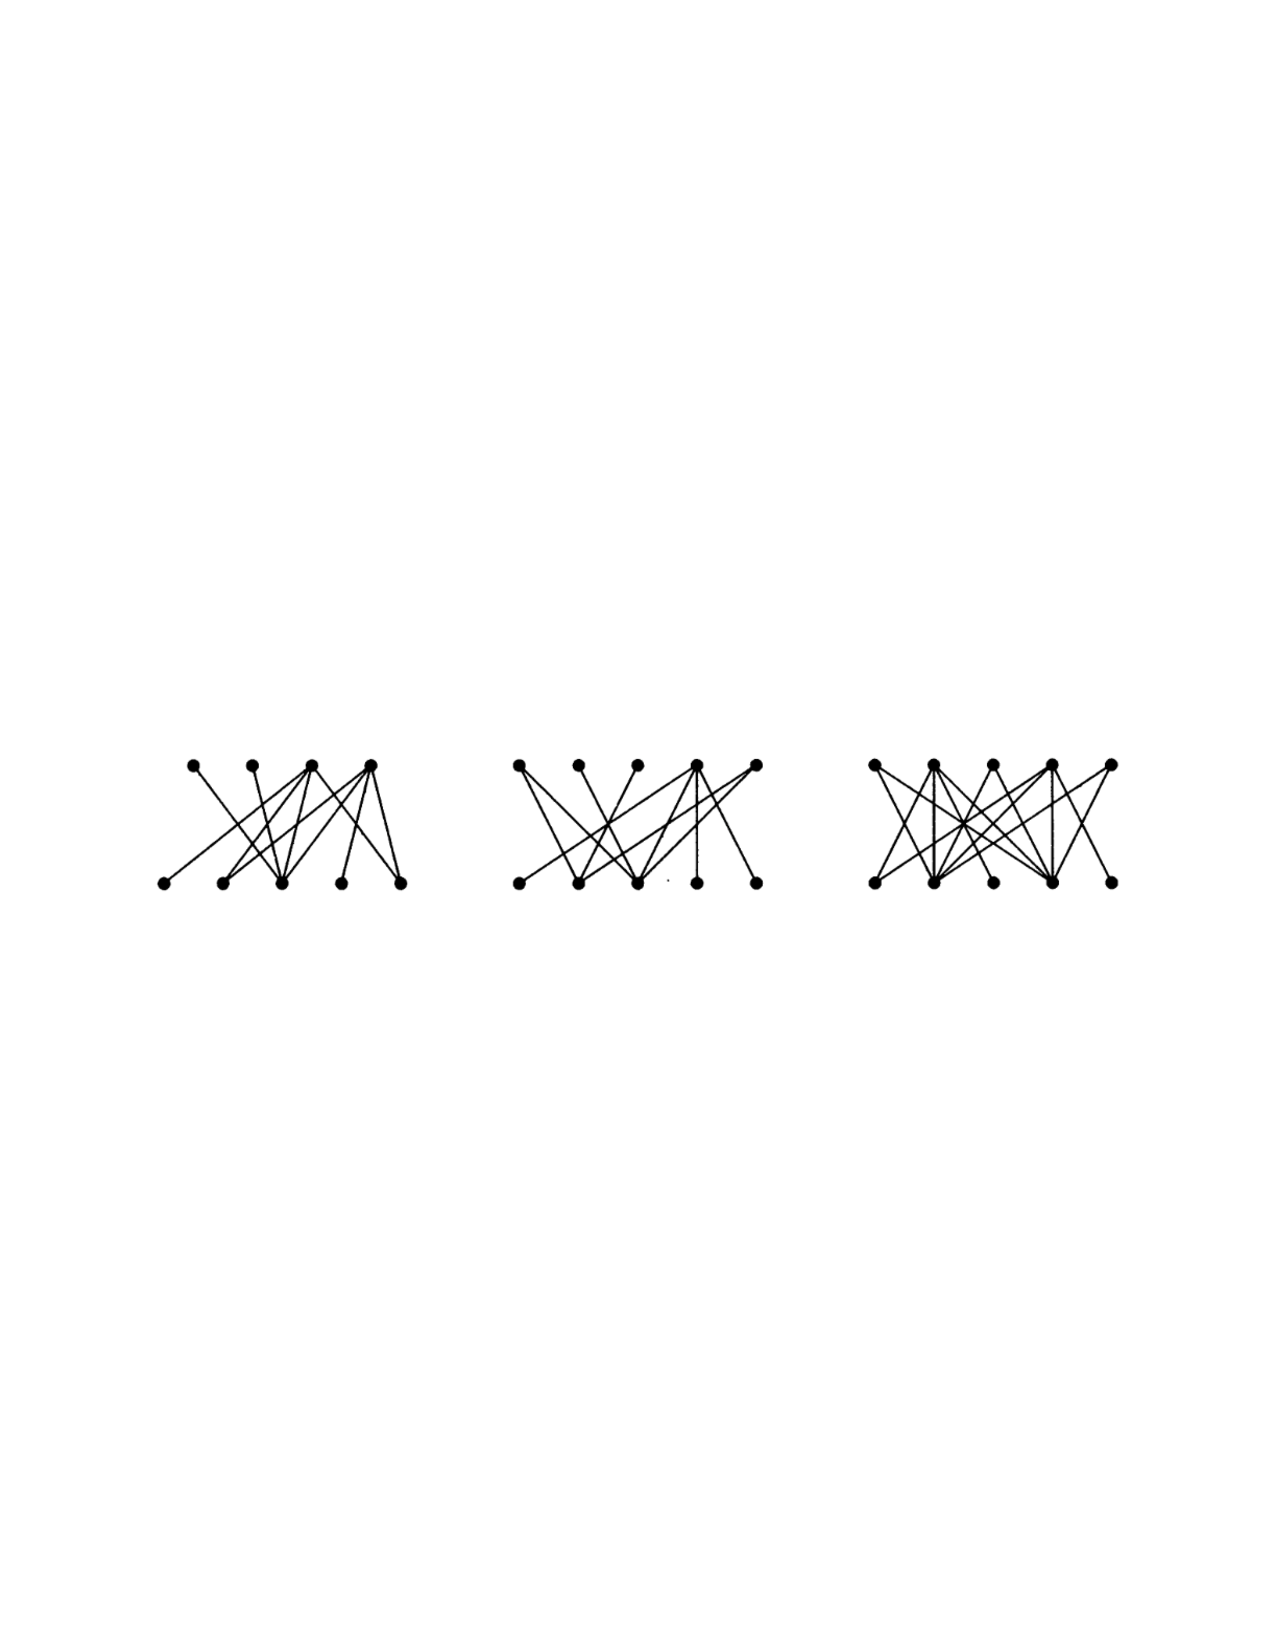
\includegraphics[scale=.8]{matchings.pdf}
\end{center}
\end{problem}

\begin{proof}

\end{proof}



\begin{problem}
Prove or disprove: every tree $T$ has at most one perfect matching. 
\end{problem}

\begin{proof}

\end{proof}


\begin{problem}
Construct a $3$-regular graph with an even number of vertices and no perfect matching. Give proof that your graph has the desired property. 
\end{problem}

\begin{proof}

\end{proof}

\begin{problem}
Two people play a game on a graph $G$, alternatively choosing distinct vertices. Player $1$ starts by choosing any vertex. Each subsequent choice must be adjacent to the preceding choice (of the other player). Thus together they follow a path. The last player able to move wins. Prove: (i) if $G$ has a perfect matching, then the second player has a winning strategy; (ii) if $G$ has no perfect matching, then the first player has a winning strategy.\footnote{Hint: think about our proof of Hall's theorem.} 
\end{problem}

\begin{proof}

\end{proof}

\begin{problem}
A permutation matrix $P$ has exactly one $1$ in each row and column and the remaining entries are $0$.  Prove that a square matrix of nonnegative integers can be expressed as the sum of $k$ permutation matrices if and only if all the row sums and column sums equal $k$. \footnote{Hint: it may help to consider graphs with multiple edges. }
\end{problem}

\begin{proof}

\end{proof}

\begin{problem}[Bonus] Use Problem 5 construct your own original $4\times 4$ magic square.\footnote{First look up what a magic square is...} Make sure the diagonals also have the same value (you will need to think about how to ensure this). Also your example should not be boring.
\end{problem}

\begin{proof}

\end{proof}





\end{document}